\documentclass[11pt]{beamer}
\usetheme{Antibes}
\usepackage[utf8]{inputenc}
\usepackage[german]{babel}
\usepackage[T1]{fontenc}
\usepackage{amsmath}
\usepackage{amsfonts}
\usepackage{amssymb}
\usepackage{graphicx}
%\author{}
%\title{}
%\setbeamercovered{transparent} 
%\setbeamertemplate{navigation symbols}{} 
%\logo{} 
%\institute{} 
%\date{} 
%\subject{} 
\begin{document}

\section{Dichtigkeitsmessung}

\subsection{Aufbau}
\begin{frame}
\begin{figure}[H]
\centering
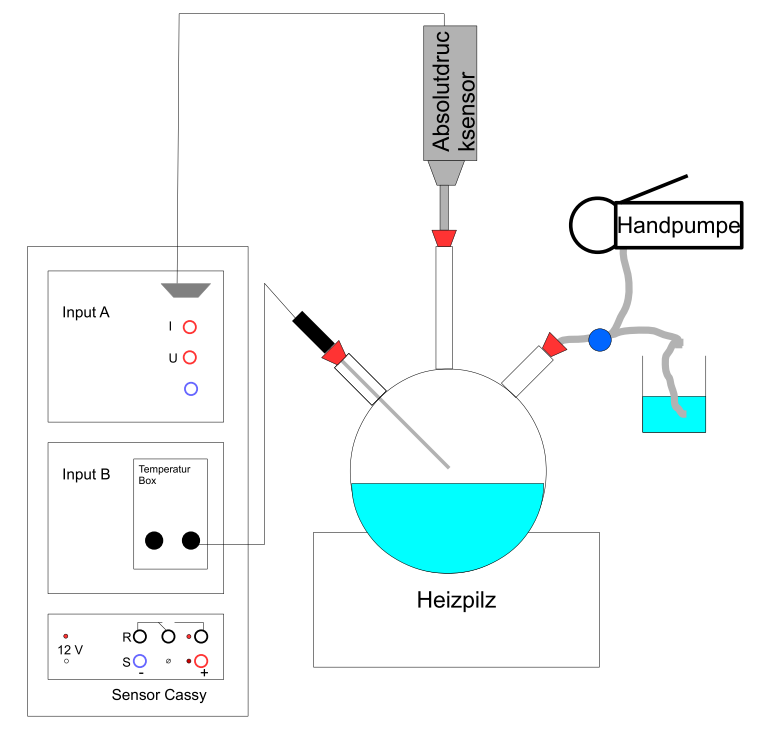
\includegraphics[scale=0.5]{Bilder/Versuchsskizze.PNG}
\end{figure}

\end{frame}

\subsection{Rohdaten}
\begin{frame}
\begin{figure}[H]
\centering
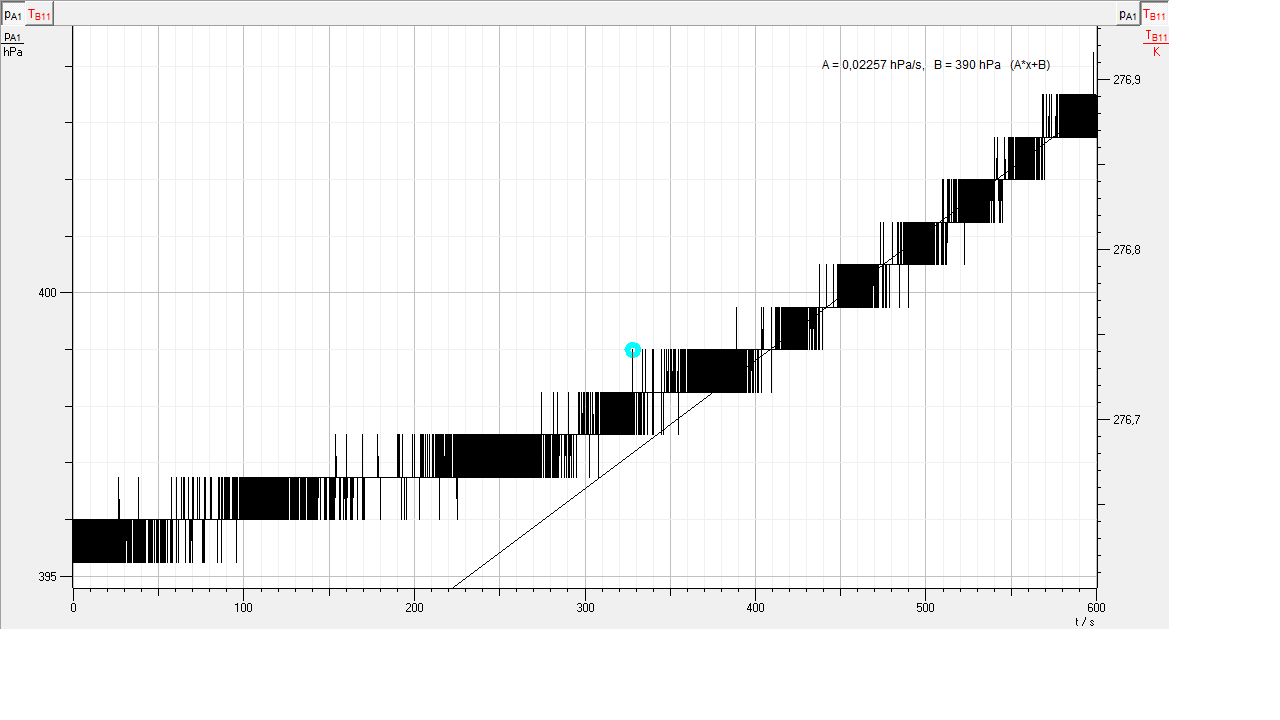
\includegraphics[scale=0.3]{Bilder/dichtigkeit_raw_JM.png}
\caption{Leckmessung Gruppe 1}
\end{figure}
\end{frame}

\begin{frame}
\begin{figure}[H]
\centering
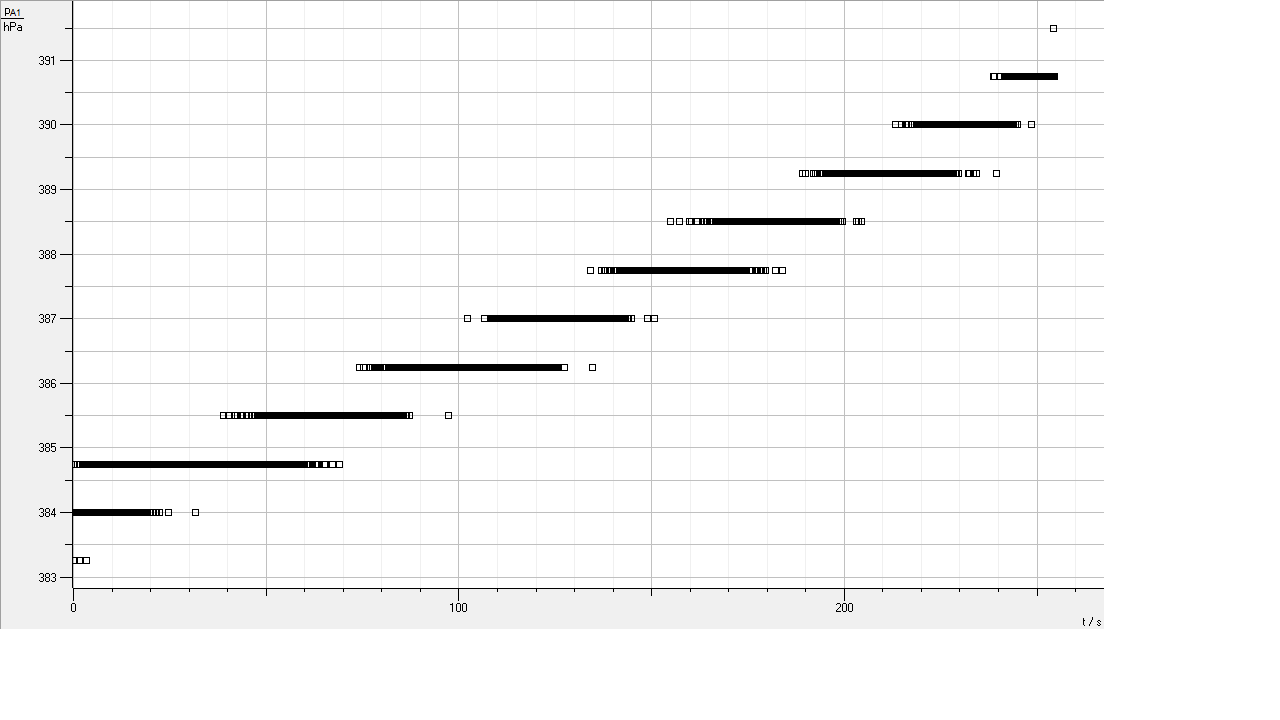
\includegraphics[scale=0.3]{Bilder/dichtigkeit_raw_EL.png}
\caption{Leckmessung Gruppe 2}
\end{figure}
\end{frame}

\subsection{Transformation der Rohdaten}
\begin{frame}
\begin{figure}[H]
\centering
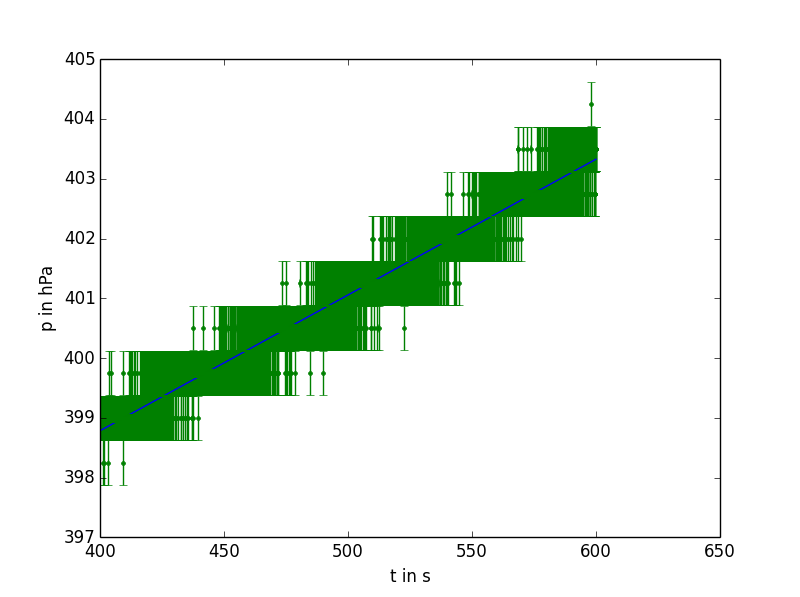
\includegraphics[scale=0.5]{Bilder/dichtigkeit__JM.png}
\caption{Lineare Regression Gruppe 1 $\frac{\chi^2}{f}=0.638$}
\end{figure}
Die Leckrate für Gruppe 1 beträgt 1.364$\,\frac{hPa}{min}$.
\end{frame}

\begin{frame}
\begin{figure}[H]
\centering
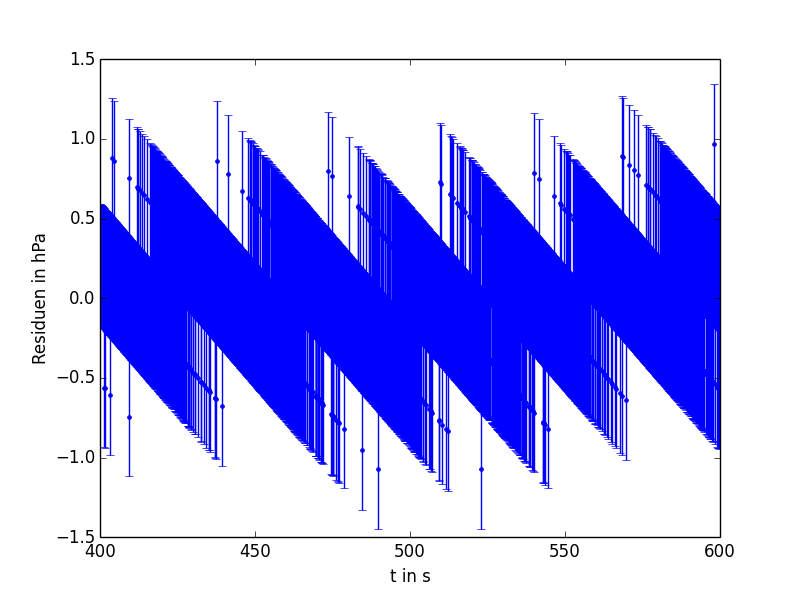
\includegraphics[scale=0.5]{Bilder/residuen_dichtigkeit_JM.png}
\caption{Residuen für die Anpassung von Gruppe 1}
\end{figure}
\end{frame}

\begin{frame}
\begin{figure}[H]
\centering
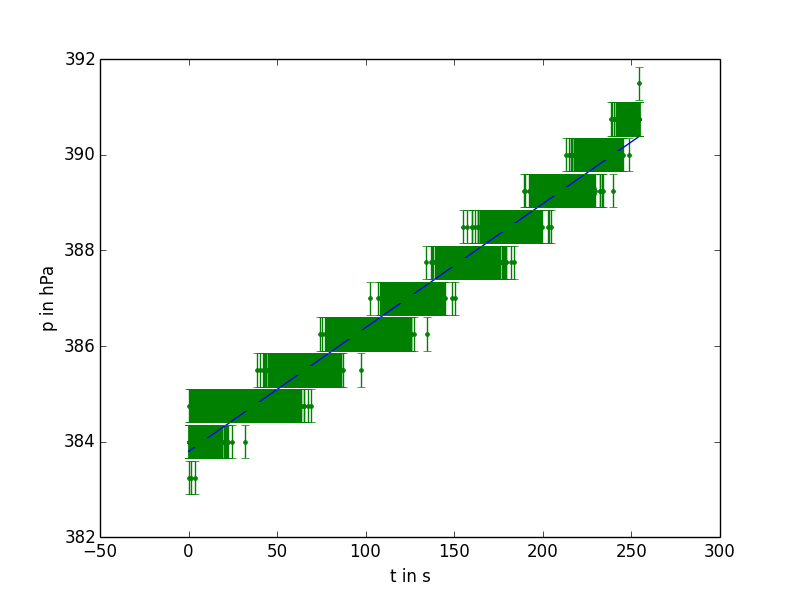
\includegraphics[scale=0.5]{Bilder/dichtigkeit__EL.png}
\caption{Lineare Regression Gruppe 2, $\frac{\chi^2}{f}=0.804$}
\end{figure}
Die Leckrate für Gruppe 2 beträgt 1.554$\,\frac{hPa}{min}$.
\end{frame}

\begin{frame}
\begin{figure}[H]
\centering
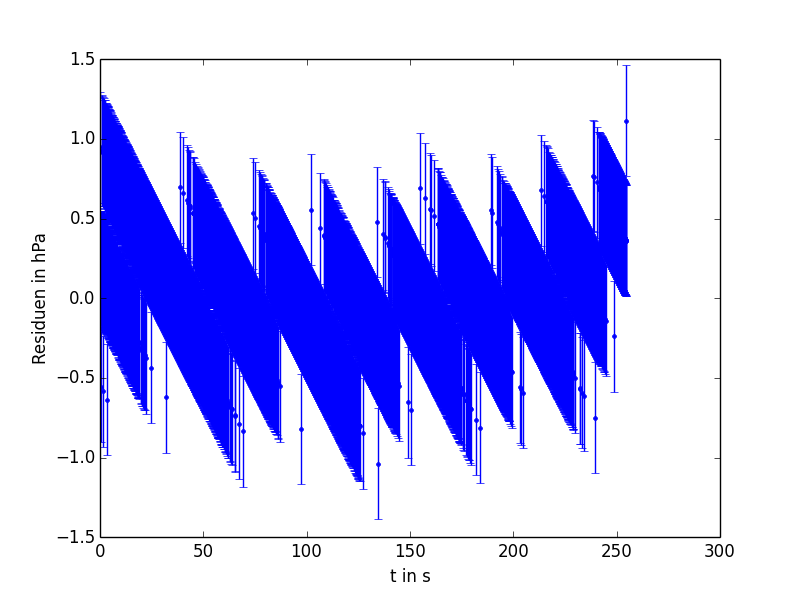
\includegraphics[scale=0.5]{Bilder/residuen_dichtigkeit_EL.png}
\caption{Residuen der Anpassung Gruppe 2}
\end{figure}
\end{frame}
\begin{frame}
fazit hier?
\end{frame}
\end{document}